\documentclass[review]{elsarticle}

\usepackage{lineno,hyperref}
\modulolinenumbers[5]

\journal{Computers \& Mathematics with Applications}

%%%%%%%%%%%%%%%%%%%%%%%
%% `Elsevier LaTeX' style
\bibliographystyle{elsarticle-num}
%%%%%%%%%%%%%%%%%%%%%%%

\usepackage{graphicx}
\usepackage{amsmath}
%\usepackage{amsfonts}
\usepackage{amssymb}
\usepackage{color}
%\usepackage{float}
\usepackage{mathtools}
\usepackage{verbatim}

\newcommand{\pdv}[2]{\frac{\partial{#1}}{\partial{#2}}}
\newcommand{\fp}[2]{\pdv{#1}{#2}}
\newcommand{\pdwc}[3]{\left(\fp{#1}{#2}\right)_{#3}}
%\newcommand{\ppdv}[3]{\displaystyle \frac{\partial^2 #1}{\partial #2\partial #3}}
\newcommand{\ppdv}[3]{\frac{\partial^2 #1}{\partial #2\partial #3}}
\newcommand{\oover}[1]{\ensuremath{\frac{1}{#1}}}

\newcommand{\vect}[1]{\boldsymbol{#1}}
\newcommand{\matr}[1]{\mathbf{#1}}
\newcommand{\dI}{\text{d}}
\newcommand{\odv}[2]{\frac{\dI #1}{\dI #2}}
\newcommand{\ddv}[2]{\odv{#1}{#2}}
%\newcommand{\ddv}[2]{\frac{\Delta #1}{\Delta #2}}
\newcommand{\nue}{\nu_{e}}
\newcommand{\nutot}{\nu_{t}}
\newcommand{\vmag}{v}
\newcommand{\vn}{\vect{n}}
\newcommand{\E}{\vect{E}}
\newcommand{\B}{\vect{B}}
\newcommand{\tE}{\vect{\tilde{E}}}
\newcommand{\tB}{\vect{\tilde{B}}}
\newcommand{\qe}{q_e}
\newcommand{\me}{m_e}
\newcommand{\fM}{f_M}
\newcommand{\fzero}{f_0}
\newcommand{\vfzero}{\vect{f}_0}
\newcommand{\fone}{\vect{f}_1}
\newcommand{\SM}{\vect{S}_M}
\newcommand{\MI}{\matr{I}}
\newcommand{\MA}{\matr{A}}
\newcommand{\intO}{\int_{\Omega}}
\newcommand{\IM}{\boldsymbol{\mathcal{M}}}
\newcommand{\ID}{\boldsymbol{\mathcal{D}}}
\newcommand{\IV}{\boldsymbol{\mathcal{V}}}
\newcommand{\IB}{\boldsymbol{\mathcal{B}}}

\newcommand{\figref}[1]{FIG.~\ref{#1}}
\renewcommand{\refeq}[1]{(\ref{#1})}

%%\renewcommand{\floatpagefraction}{.9}% 
%\newlength{\picwidth}
%\setlength{\picwidth}{0.49\linewidth}
%%\setlength{\picwidth}{11cm}

%%%%%%%%%%%%%%%%%%%%%%%
\begin{document}

\begin{frontmatter}

\title{High-order finite element modeling of M1-AWBS nonlocal electron transport}
%\tnotetext[mytitlenote]{}

\author[celiaaddress]{Milan, Vladimir, Philippe, Jean-Luc}
\address[celiaaddress]{Universit\'{e} de Bordeaux - CNRS - CEA, CELIA, UMR 5107, F-33405 Talence, France}


\begin{abstract}

\end{abstract}

\begin{keyword}
Nonlocal transport \sep Kinetics \sep MHD \sep High-order methods \sep FEM
%\MSC[2010] 00-01\sep  99-00
\end{keyword}

\end{frontmatter}

\linenumbers

%---------------------------------------------------------------------
%---------------------------------------------------------------------

\fbox{\parbox{0.99\textwidth}{
%\centerline{\textcolor{red}{THIS WILL BE REMOVED}}
\footnotesize
\tableofcontents
}}
\newpage

%---------------------------------------------------------------------
%---------------------------------------------------------------------
%\section{Moments method}\label{sec:moment_method}

\section{M1 model}\label{sec:m1_model}
\subsection{AWBS Boltzmann transport equation}
Simplified Boltzmann transport equation of electrons relying on the use of AWBS
collision-thermalization operator \cite{AWBS_PRL1986} reads
\begin{equation}
  \vmag\vn\cdot\nabla f + \frac{\qe}{\me}\left( \E + 
  \frac{\vmag}{c}\vn\times\B\right)\cdot\nabla_{\vect{v}} f = \nue \vmag 
  \pdv{}{\vmag}\left( f - \fM\right) .
  \label{eq:AWBS}
\end{equation}
\subsection{M1-AWBS model}
In order to eliminate the~dimensions of the~transport problem \refeq{eq:AWBS}
the~two moment model referred to as \textit{M1-AWBS} is introduced
\begin{eqnarray}
  \nue\vmag\pdv{}{\vmag}\left(\fzero - \fM \right) &=&
  \vmag\nabla\cdot\fone + \frac{\qe}{\me\vmag^2}\E\cdot\pdv{}{\vmag}
  \left( \vmag^2 \fone\right) , 
  \label{eq:M1f0}\\
  \nue\vmag\pdv{}{\vmag}\fone - \nutot\fone &=& 
  \vmag\nabla\cdot\left(\MA\fzero\right) + 
  \frac{\qe}{\me\vmag^2}\E\cdot\pdv{}{\vmag}
  \left( \vmag^2 \MA\fzero\right) \nonumber\\
  && + \frac{\qe}{\me\vmag}\E\cdot\left( \MA - \MI \right)\fzero +
  \frac{\qe}{\me c}\B\times\fone ,
  \label{eq:M1f1}
\end{eqnarray}
where the~anisotropy-closure matrix takes the~form
\begin{equation}
  \MA = \frac{1}{3}\MI + \frac{|\fone|^2}{2\fzero^2}
  \left( 1 + \frac{|\fone|^2}{\fzero^2} \right)
  \left( \frac{\fone\otimes\fone^T}{|\fone|^2} - \frac{1}{3}\MI\right) .
\end{equation}
%---------------------------------------------------------------------
\section{High-order finite element scheme}\label{sec:hos}
\begin{comment}
\begin{eqnarray}
  \rho \pdv{\fzero}{\vmag} &=& 
  \frac{\rho}{\nue}\MI:\nabla\fone + 
  \frac{\qe\rho}{\me\nue\vmag}\E\cdot\pdv{\fone}{\vmag}
  + \frac{2 \qe\rho}{\me\nue\vmag^2}\E\cdot\fone + \rho \pdv{\fM}{\vmag} , 
  \label{eq:M1hosf0}\\
  \rho \pdv{\fone}{\vmag} &=&
  %\frac{\rho}{\nue}\nabla\cdot\left(\MA\fzero\right) + 
  \nabla\cdot\left(\frac{\rho\MA}{\nue}\fzero\right) +
  \left(\frac{\qe\rho}{\me\nue\vmag^2}\E\cdot\left( 3\MA - \MI \right) - 
  \nabla\left( \frac{\rho}{\nue}\right)\cdot\MA \right)\fzero \nonumber\\
  &&+ \frac{\qe\rho}{\me\nue\vmag}\E\cdot\pdv{}{\vmag}
  \left( \MA\fzero\right) + \frac{\qe\rho}{\me c \nue\vmag}\B\times\fone + 
  \frac{\rho \nutot}{\nue\vmag}\fone .
  \label{eq:M1hosf1}
\end{eqnarray}
\end{comment}
\subsection{Variational principle}
First, the~electro-magnetic scaling
\begin{equation}
  \tE = \frac{\qe}{\me}\E,~\tB = \frac{\qe}{\me c} \B,
\end{equation}
is defined in order to make the~algebraic operations easier to follow.
The~general variational formulation of \eqref{eq:M1f0} and \eqref{eq:M1f1} 
constructed above the~scalar (zero moment) functional space
represented by test functions $\phi$ and the~vector
(first moment) functional space represented by test functions $\vect{w}$ 
takes the~form
\begin{eqnarray}
  \intO\phi\rho \pdv{\fzero}{\vmag} &=& 
  \intO\phi
  \left(\frac{\rho}{\nue}\MI:\nabla\fone + 
  \frac{\rho}{\nue\vmag}\tE\cdot\pdv{\fone}{\vmag}
  + \frac{2 \rho}{\nue\vmag^2}\tE\cdot\fone + \rho \pdv{\fM}{\vmag}\right) , 
  \label{eq:M1hosf0_variational}\\
  \intO\vect{w}\cdot\rho \pdv{\fone}{\vmag} &=&
  %\frac{\rho}{\nue}\nabla\cdot\left(\MA\fzero\right) + 
  \intO\vect{w}\cdot\Bigg(\nabla\cdot\left(\frac{\rho\MA}{\nue}\fzero\right) 
  - \nabla\left( \frac{\rho}{\nue}\right)\cdot\MA\fzero 
  + \frac{\rho}{\nue\vmag^2}\tE\cdot\left( 3\MA - \MI \right)\fzero
  \nonumber\\
  && 
  + \frac{\rho}{\nue\vmag}\tE\cdot\pdv{}{\vmag}
  \left( \MA\fzero\right) + \frac{\rho}{\nue\vmag}\tB\times\fone + 
  \frac{\rho \nutot}{\nue\vmag}\fone\Bigg) .
  \label{eq:M1hosf1_variational}
\end{eqnarray}

The~corresponding discrete variational principal based on the~method of 
finite elements then reads
\begin{multline}
  \intO\vect{\phi}\, \otimes\, \vect{\phi}^T 
  \rho\, \dI \Omega \cdot \pdv{\vfzero}{\vmag} = 
  \intO\vect{\phi}\, \otimes \left(
  \frac{\rho}{\nue}\MI:\nabla\matr{w}^T + 
  \frac{2 \rho}{\nue\vmag^2}\tE^T \cdot\matr{w}^T \right)\dI \Omega
  \cdot \fone \\
  + \intO\vect{\phi}\, \otimes
  \frac{\rho}{\nue\vmag}\tE^T \cdot \matr{w}^T\, \dI \Omega 
  \cdot \pdv{\fone}{\vmag} + 
  \intO\vect{\phi}\, \otimes\, \vect{\phi}^T \rho\, \dI\Omega\,
  \cdot \pdv{\vect{\fM}}{\vmag} , 
  \label{eq:FEM1hosf0}
\end{multline}
\begin{multline}
  \intO\matr{w} \cdot \matr{w}^T \rho\, \dI\Omega \cdot 
  \pdv{\fone}{\vmag} =
  - \intO
  \left(\frac{\rho}{\nue} \MA : \nabla\matr{w} 
  + \matr{w} \cdot \MA \cdot \nabla\left(\frac{\rho}{\nue}\right)\right)
  \vect{\phi}^T\, \dI \Omega\, 
  \cdot \vfzero \\
  + \intO\matr{w} \cdot 
  \frac{\rho}{\nue\vmag^2} \left( 3\MA - \MI \right) \cdot \tE\,  
  \vect{\phi}^T\, \dI\Omega \cdot \vfzero 
  + \intO\matr{w} \cdot
  \frac{\rho}{\nue\vmag} \MA \cdot \tE\, \vect{\phi}^T\, \dI \Omega 
  \cdot \pdv{\vfzero}{\vmag}\\
  + \intO\matr{w} \cdot
  \left(\frac{\rho}{\nue\vmag}\tilde{\B}\times\matr{w}^T + 
  \frac{\rho \nutot}{\nue\vmag} \matr{w}^T\right)\, \dI\Omega 
  \cdot \fone ,
  \label{eq:FEM1hosf1}
\end{multline}
where $\vect{\phi}$ is the~finite vector of scalar bases functions, 
$\matr{w}$ is the~finite vector of vector bases functions,
$\Omega$ represents the~computational domain, in principle 1D/2D/3D 
spatial mesh. 

\subsection{Semi-discrete formulation}\label{sec:semidiscrete_form}

In principle, only five following integrators need to be coded to provide
a~discrete representation \eqref{eq:FEM1hosf0} and \eqref{eq:FEM1hosf1}, i.e.
\begin{eqnarray}
  \IM^0_{(g)} &=& \intO\vect{\phi}\, \otimes\, \vect{\phi}^T g\, \dI \Omega ,
  \label{eq:IM0}\\
  \IM^1_{(g)} &=& \intO\matr{w} \cdot \matr{w}^T g\, \dI\Omega ,
  \label{eq:IM1}\\
  \ID_{(\matr{G})} &=& \intO \matr{G} : \nabla\matr{w}
  \, \otimes\, \vect{\phi}^T\, \dI \Omega ,
  \label{eq:ID}\\
  \IV_{(\vect{g})} &=& \intO\matr{w} \cdot
  \vect{g}\, \otimes\, \vect{\phi}^T\, \dI \Omega ,
  \label{eq:IV}\\
  \IB_{(\vect{g})} &=& \intO\matr{w} \cdot
  \vect{g} \times \matr{w}^T\, \dI \Omega .
  \label{eq:IB}
\end{eqnarray}
The~algebraic representation of the~above mathematical objects, which
form the~basis for numerical discretization, reads 
\begin{equation}
  \vect{\phi} = \begin{bmatrix}
    \phi_{1} \\
	\vdots   \\
	\phi_{N_0}
  \end{bmatrix},~
  \matr{w} = \begin{bmatrix}
    w_{1, 1} & \hdots & w_{1, d} \\
	\vdots   & \ddots & \vdots \\
	w_{N_1, 1} & \hdots & w_{N_1, d}
  \end{bmatrix},~
  \vect{g} = \begin{bmatrix}
    g_{1} \\
	\vdots   \\
	g_{d}
  \end{bmatrix},~
  \matr{G} = \begin{bmatrix}
    G_{1, 1} & \hdots & G_{1, d} \\
	\vdots   & \ddots & \vdots \\
	G_{d, 1} & \hdots & G_{d, d}
  \end{bmatrix},
\end{equation}
where $d$ is the~number of spatial dimensions, $N_0$ the~number of
degrees of freedom of scalar unknown $\vfzero$, and $N_1$ is the~number
of degrees of freedom of vector unknown $\fone$.

Consequently, the~discrete analog of M1-AWBS equations
\eqref{eq:M1f0} and \eqref{eq:M1f1} can be written based on 
 \eqref{eq:FEM1hosf0}, \eqref{eq:FEM1hosf1} as
\begin{multline}
  \IM^0_{(\rho)} \cdot \pdv{\vfzero}{\vmag} 
  - \IM^0_{(\rho)} \cdot \pdv{\vect{\fM}}{\vmag}
  = 
  \ID^T_{\left(\frac{\rho}{\nue}\MI\right)} \cdot \fone
  + \frac{1}{\vmag}\IV^T_{\left(\frac{\rho}{\nue}\tE\right)} \cdot 
  \pdv{\fone}{\vmag} 
  + \frac{2}{\vmag^2}\IV^T_{\left(\frac{\rho}{\nue}\tE\right)} \cdot \fone ,  
  \label{eq:semiM1hosf0}
\end{multline}
\begin{multline}
  \IM^1_{(\rho)} \cdot \pdv{\fone}{\vmag} 
  - \frac{1}{\vmag}\IM^1_{\left( \frac{\rho \nutot}{\nue} \right)} 
  \cdot \fone 
  = 
  - \left(\ID_{\left(\frac{\rho}{\nue}\MA\right)}  
  + \IV_{\left( \MA \cdot \nabla\left(\frac{\rho}{\nue}\right) \right)}\right) 
  \cdot \vfzero \\ 
  + \frac{1}{\vmag}\IV_{\left(\frac{\rho}{\nue}\MA \cdot \tE\right)} \cdot
  \pdv{\vfzero}{\vmag}
  + \frac{1}{\vmag^2}\IV_{\left(\frac{\rho}{\nue} 
  \left( 3\MA - \MI \right) \cdot \tE \right)} \cdot \vfzero
  + \frac{1}{\vmag}\IB_{\left( \frac{\rho}{\nue}\tB \right)} \cdot \fone ,
  \label{eq:semiM1hosf1}
\end{multline}
where the~integrators \eqref{eq:IM0}, \eqref{eq:IM1},
\eqref{eq:ID}, \eqref{eq:IV}, \eqref{eq:IB} are used acting on appropriate
functions $\rho$, $\nue$, $\nutot$, vectors $\tE$, $\tB$, and matrices $\MA$
and $\MI$.

Also, it proves to be useful to define mass matrices
\begin{equation}
  \matr{M}_0^c = \IM^0_{(\rho)},~\matr{M}_1^c = \IM^1_{(\rho)} ,
  \label{eq:massmatrices} 
\end{equation}
since these are constant during the~time evolution of the~Lagrangian mesh,
thus making the~overall matrix evaluation more efficient.

\subsection{Explicit fully-discrete scheme}\label{sec:expl_fullydiscrete_scheme}
The~easiest way to define a~fully discrete scheme is to apply the~explicit
integration in time, e.g. RK4.
Because of the~use of different finite element spaces for zero and first moment,
and a~consequent difficulties of "mass" inversion, a~modified two-step explicit
scheme is used.

In the~first step the~time evolution of zero moment quantity $\vfzero$ is 
computed as
\begin{multline}
  \left( \matr{M}^c_0 
  - \frac{1}{\vmag}
  \IV^T_{\left(\frac{\rho}{\nue\vfzero^n}\tE^T\cdot\fone^n\right)}
  \right) \cdot {\ddv{\vfzero}{\vmag}}^* 
  = 
  \ID^T_{\left(\frac{\rho}{\nue}\MI\right)} \cdot \fone^n 
  + \frac{2}{\vmag^2}\IV^T_{\left(\frac{\rho}{\nue}\tE\right)} \cdot \fone^n
  + \matr{M}^c_0 \cdot \pdv{\vect{\fM}}{\vmag} ,  
  \label{eq:explM1hosf0}
\end{multline}
where the~actual evolution of $\fone$ has been redefined as similar to 
the~time evolution of $\vfzero$ (compare \eqref{eq:explM1hosf0} to 
\eqref{eq:semiM1hosf0}). Then, the~actual computation of the~time evolution 
of $\fone$ follows
\begin{multline}
  \matr{M}^c_1 \cdot \ddv{\fone}{\vmag} 
  = 
  - \left(\ID_{\left(\frac{\rho}{\nue}\MA\right)}  
  + \IV_{\left( \MA \cdot \nabla\left(\frac{\rho}{\nue}\right) \right)} \right) 
  \cdot \vfzero^n  
  + \frac{1}{\vmag}\IV_{\left(\frac{\rho}{\nue}\MA \cdot \tE\right)} \cdot
  {\ddv{\vfzero}{\vmag}}^* \\
  + \frac{1}{\vmag^2}\IV_{\left(\frac{\rho}{\nue} 
  \left( 3\MA - \MI \right) \cdot \tE \right)} \cdot \vfzero^n
  + \frac{1}{\vmag}\IB_{\left( \frac{\rho}{\nue}\tB \right)} \cdot \fone^n
  + \frac{1}{\vmag}\IM^1_{\left( \frac{\rho \nutot}{\nue} \right)} 
  \cdot \fone^n .
  \label{eq:explM1hosf1}
\end{multline}
The~superscript $n$ stands for quantities from the~previous level of velocity.

\begin{figure}[tbh]
  \begin{center}
    %\begin{tabular}{c}
      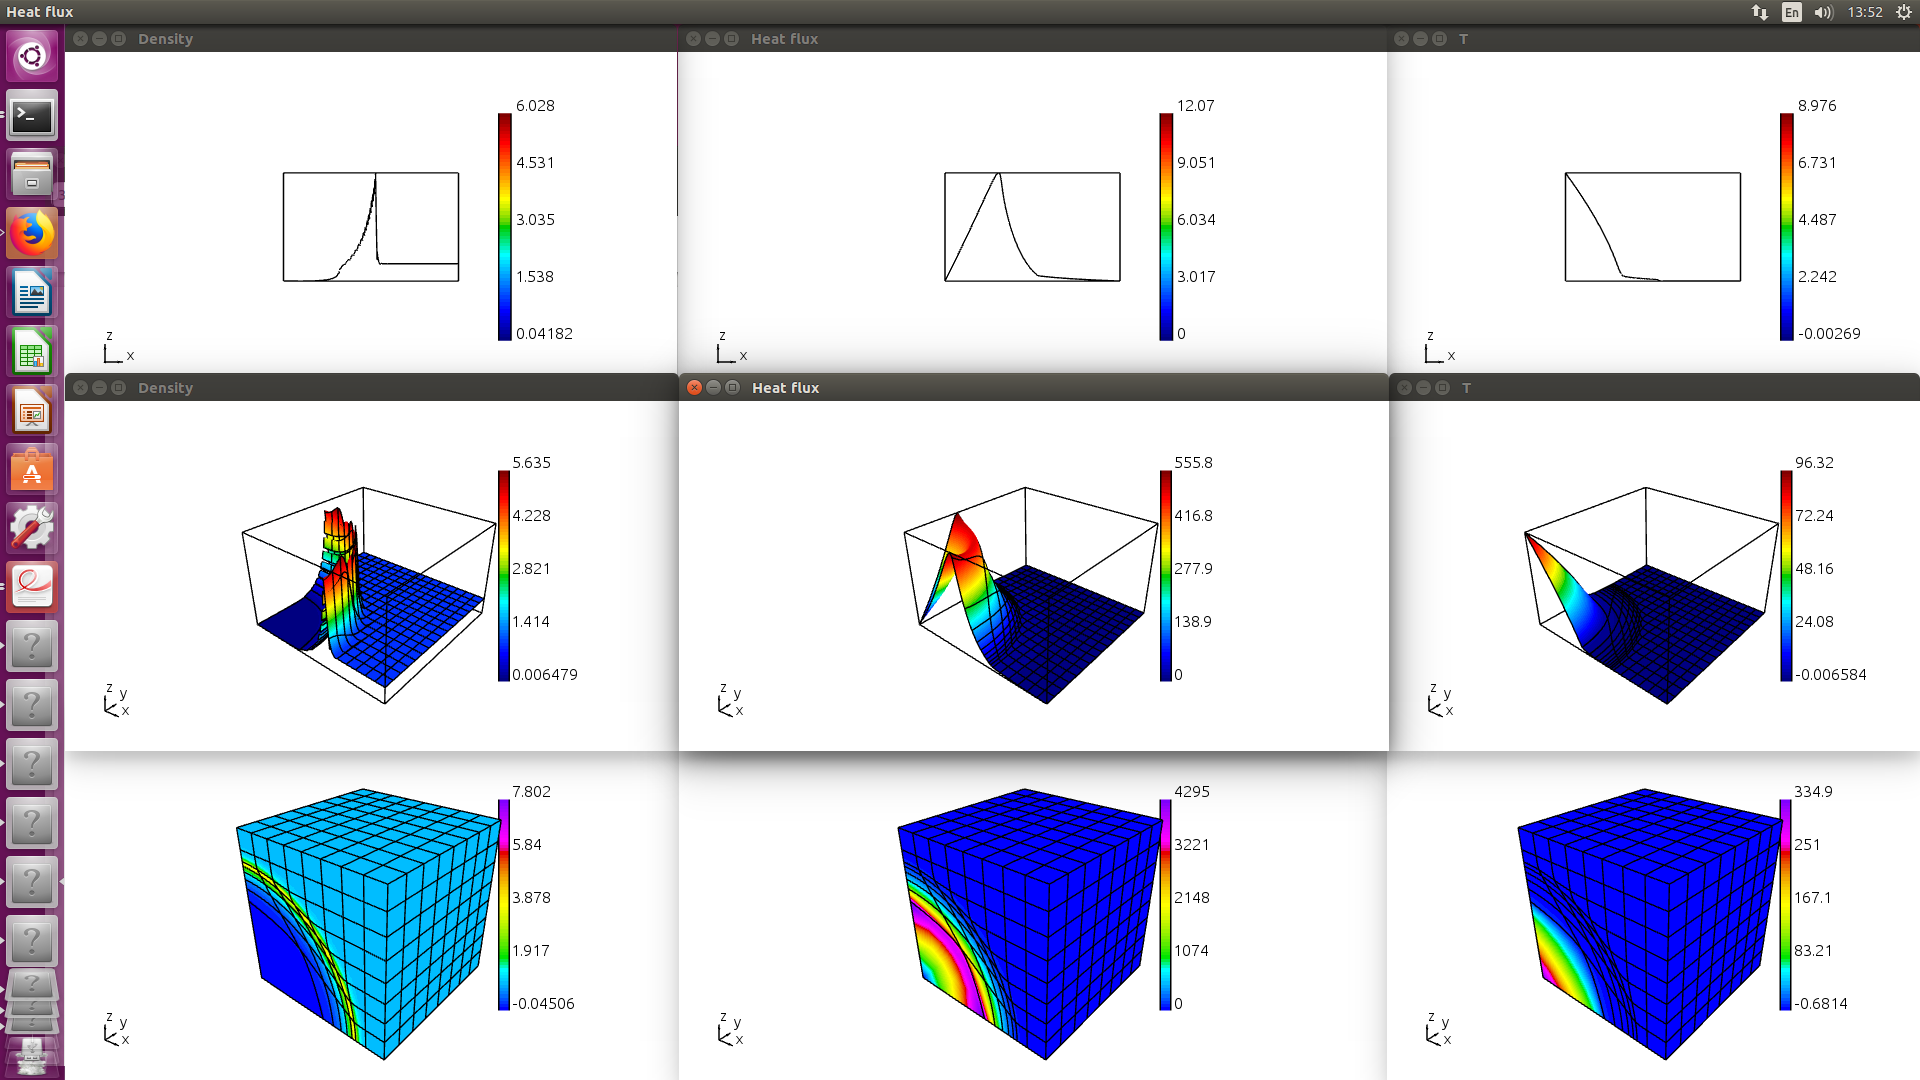
\includegraphics[width=1.0\textwidth]{M1Sedov1D2D3D.png}
    %\end{tabular}
  \caption{
  Sedov blast in 1D/2D/3D from $\delta$ function hot spot. 
  Shock propagates from left to right. Top raw corresponds to 1D 
  (8858 energy groups) - 
  left: density profile, right: temperature 
  (decreasing from the~original hot spot with low temperature in compressed 
  plasma), center: heat flux with its maximum on the~start of increase 
  in density decreasing while approaching the~shock 
  (NOTICE non-zero flux ahead of the~shock). 
  Middle raw corresponds to 2D (4348 energy groups) - 
  left: density, center: heat flux, right: temperature.
  Bottom raw corresponds to 3D (10030 energy groups) - 
  left: density, center: heat flux, right: temperature.
  temperature 
  }
  \end{center}
  \label{fig:expl1D2D3D}
\end{figure}

As can be seen in \figref{fig:expl1D2D3D} we get a~heat flux profile 
corresponding to temperature and density profiles computed by Laghos 
\cite{Dobrev_Kolev_Rieben-High-order_curvilinear_finite_element_methods_for_Lagrangian_hydrodynamics}
in 1D and we have also double checked the~numerical scheme in 2D and 3D, where
apparently the~flux profiles exhibit the~same physical background.
It is important to note, that the~current implementation does not include
neither electric or magnetic field ($\tE$, $\tB$).

It is worth mentioning, that the~proposed discrete scheme 
\eqref{eq:explM1hosf0} and \eqref{eq:explM1hosf1} naturally obeys the~CFL
condition with respect to the~mesh smallest cell size/mean-stopping-power, and
consequently, we needed 8858 energy groups in 1D, 4348 energy groups in 2D, and
10030 energy groups in 3D. This would make the~hydro simulation to take 
more than 1000x longer than classical (SH) hydro.

\subsection{Implicit fully-discrete scheme}\label{sec:impl_fullydiscrete_scheme}
In order to formulate a~fully-discrete scheme leaning on an~implicit 
discretization of velocity, the~equations \eqref{eq:semiM1hosf0} and 
\eqref{eq:semiM1hosf1} can be expressed with matrices as
\begin{eqnarray}
  \matr{M}^c_0 \cdot \pdv{\vfzero}{\vmag}  
  &=& 
  \matr{D}_0 \cdot \fone
  + \matr{E}_0^1 \cdot \pdv{\fone}{\vmag} + \matr{E}_0^2 \cdot \fone
  + \matr{M}^c_0 \cdot \pdv{\vect{\fM}}{\vmag} ,  
  \nonumber\\
  \matr{M}^c_1 \cdot \pdv{\fone}{\vmag}  
  &=& 
  - \matr{D}_1 \cdot \vfzero 
  + \matr{E}_1^1 \cdot \pdv{\vfzero}{\vmag}
  + \matr{E}_1^2 \cdot \vfzero
  + \matr{B} \cdot \fone
  + \matr{M}_1 \cdot \fone ,
  \nonumber
\end{eqnarray}

\begin{eqnarray}
  \ddv{\vfzero}{\vmag}  
  &=& 
  {\matr{M}^c_0}^{-1} \cdot \left(\matr{D}_0 + \matr{E}_0^2 \right) 
  \cdot \left(\fone^n + \Delta \vmag \ddv{\fone}{\vmag} \right)
  + {\matr{M}^c_0}^{-1} \cdot \matr{E}_0^1 \cdot \ddv{\fone}{\vmag} \nonumber\\
  && + \pdv{\vect{\fM}}{\vmag} ,  
  \nonumber\\
  \matr{M}^c_1 \cdot \ddv{\fone}{\vmag}  
  &=& 
  \left( \matr{E}_1^2 - \matr{D}_1 \right) 
  \cdot \left(\vfzero^n + \Delta\vmag \ddv{\vfzero}{\vmag} \right) 
  + \matr{E}_1^1 \cdot \ddv{\vfzero}{\vmag} \nonumber\\
  && + \left( \matr{B} + \matr{M}_1 \right)  
  \cdot \left(\fone^n + \Delta \vmag \ddv{\fone}{\vmag} \right) ,
  \nonumber
\end{eqnarray}
%\begin{multline}
%  \ddv{\vfzero}{\vmag}  
%  = 
%  {\matr{M}^c_0}^{-1} \cdot \left( \Delta\vmag \left(\matr{D}_0 
%  + \matr{E}_0^2 \right) + \matr{E}_0^1 \right) \cdot \ddv{\fone}{\vmag}
%  + {\matr{M}^c_0}^{-1} \cdot \left(\matr{D}_0 + \matr{E}_0^2 \right) 
%  \cdot \fone^n
%  + \pdv{\vect{\fM}}{\vmag}~,  
%  \nonumber
%\end{multline}

%\begin{multline}
%  \left( \matr{M}^c_1 
%  - \Delta \vmag \left( \matr{B} + \matr{M}_1 \right) \right) 
%  \cdot \ddv{\fone}{\vmag}  
%  = 
%  \left( \matr{E}_1^1 + 
%  \Delta\vmag\left( \matr{E}_1^2 - \matr{D}_1 \right)\right) 
%  \cdot \ddv{\vfzero}{\vmag}
%  + \left( \matr{B} + \matr{M}_1 \right)  
%  \cdot \fone^n
%  + \left( \matr{E}_1^2 - \matr{D}_1 \right)
%  \cdot \vfzero^n~, 
%  \nonumber
%\end{multline}

\begin{eqnarray}
  \ddv{\vfzero}{\vmag}  
  &=& 
  \matr{\tilde{A}}_0 \cdot \ddv{\fone}{\vmag}
  + \vect{b}_0\left(\fone^n, \pdv{\vect{\fM}}{\vmag}\right) ,  
  \label{eq:df0dv} \\
  \left( \matr{M}^c_1 
  - \Delta \vmag \left( \matr{B} + \matr{M}_1 \right) \right) 
  \cdot \ddv{\fone}{\vmag}  
  &=& 
  \matr{\tilde{A}}_1 \cdot \ddv{\vfzero}{\vmag}  
  + \vect{b}_1 \left( \fone^n, \vfzero^n \right) , 
  \label{eq:df1dvdf0dv}
\end{eqnarray}

\begin{equation}
  \left( \matr{M}^c_1 
  - \Delta \vmag \left( \matr{B} + \matr{M}_1 \right) 
  - \matr{\tilde{A}}_1 \cdot \matr{\tilde{A}}_0 \right) 
  \cdot \ddv{\fone}{\vmag}  
  = 
  \matr{\tilde{A}}_1 
  \cdot \vect{b}_0 + \vect{b}_1 , 
  %\matr{\tilde{A}}_1 
  %\cdot \vect{b}_0\left(\fone^n, \pdv{\vect{\fM}}{\vmag}\right)
  %+ \vect{b}_1 \left( \fone^n, \vfzero^n \right)~, 
  \label{eq:df1dv}
\end{equation}

\begin{comment} % old discrete analog
The~M1-AWBS model can be written as an~algebraic representation
\begin{eqnarray}
  \matr{M}_0\, \cdot\, \pdv{\vfzero}{\vmag} &=& 
  \left(\matr{D}_0^T + \frac{2}{\vmag^2}\matr{E}_0\right) \cdot\, \fone + 
  \frac{1}{\vmag}\matr{E}_0\, \cdot\, \pdv{\fone}{\vmag}
  + \matr{M}_0\, \cdot\, \pdv{\vect{\fM}}{\vmag}\, , 
  \label{eq:MM1hosf0}\\
  \matr{M}_1\, \cdot\, \pdv{\fone}{\vmag} &=& 
  - \matr{D}_1\, \cdot\, \vfzero + \matr{EI}_1\, \cdot\, \vfzero
  + \matr{E}_1\, \cdot\, \pdv{\vfzero}{\vmag} 
  + \matr{B}_1\, \cdot\, \fone + \matr{N}_1\, \cdot\, \fone\, ,
  \label{eq:MM1hosf1}
\end{eqnarray}

\begin{eqnarray}
  \matr{M}_0\, \cdot\, \ddv{\vfzero}{\vmag} &=& 
  \left(\matr{D}_0^T + \frac{2}{\vmag^2}\matr{E}_0\right) \cdot\, \fone^n + 
  \frac{1}{\vmag}\matr{E}_{1/0}\, \cdot\, \ddv{\vfzero}{\vmag}
  + \matr{M}_0\, \cdot\, \SM~,
  \label{eq:mm1hosf0_expl}\\
  \matr{M}_1\, \cdot\, \ddv{\fone}{\vmag} &=& 
  \left( \matr{EI}_1 - \matr{D}_1 \right)\, \cdot\, \vfzero^n
  + \matr{E}_1\, \cdot\, \ddv{\vfzero}{\vmag} 
  + \left(\matr{B}_1 + \matr{N}_1\right)\, \cdot\, \fone^n~,
  \label{eq:mm1hosf1_expl}
\end{eqnarray}

\begin{eqnarray}
  \matr{M}_0\, \cdot\, \ddv{\vfzero}{\vmag} &=& 
  \left(\matr{D}_0^T + \frac{2}{\vmag^2}\matr{E}_0\right) \cdot\, 
  \left( \fone^{n} + \Delta\vmag \ddv{\fone}{\vmag} \right) + 
  \frac{1}{\vmag}\matr{E}_0\, \cdot\, \ddv{\fone}{\vmag}
  + \matr{M}_0\, \cdot\, \SM~, \nonumber\\ 
  \label{eq:mm1hosf0_impl}\\
  \matr{M}_1\, \cdot\, \ddv{\fone}{\vmag} &=& 
  \left( \matr{EI}_1 - \matr{D}_1\right)\, \cdot\, 
  \left( \vfzero^{n} + \Delta\vmag\ddv{\vfzero}{\vmag} \right)
  + \matr{E}_1\, \cdot\, \ddv{\vfzero}{\vmag} \nonumber \\ 
  && + \left(\matr{B}_1 + \matr{N}_1\right)\, \cdot\, 
  \left( \fone^{n} + \Delta\vmag\ddv{\fone}{\vmag} \right)\, ,
  \label{eq:mm1hosf1_impl}
\end{eqnarray}

\begin{eqnarray}
  \matr{M}_0 &=& \int_{\Omega}\vect{\phi}\, \otimes\, \vect{\phi}^T 
  \rho\, \dI \Omega~, \\
  \matr{D}_0 &=& \int_{\Omega}\vect{\phi}\, \otimes
  \frac{\rho}{\nue}\MI:\nabla\vect{w}^T\, \dI \Omega~, \\
  \matr{E}_0 &=& \int_{\Omega}\vect{\phi}\, \otimes
  \frac{\rho}{\nue}\tilde{\E}\, \cdot\, \vect{w}^T\, \dI \Omega~, \\
  \matr{E}_{1/0} &=& \int_{\Omega}
  \frac{\rho}{\nue\fzero^n}\tilde{\E}\, \cdot\, \fone^n\,
  \vect{\phi}\, \otimes\, \vect{\phi}^T\, \dI \Omega~.
\end{eqnarray}

\begin{eqnarray}
  \matr{M}_1 &=& \int_{\Omega}\vect{w}\, \otimes\, \vect{w}^T \rho\, \dI\Omega~,  \\
  \matr{D}_1 &=& \int_{\Omega}\frac{\rho}{\nue} \MA : \nabla\vect{w}\, \otimes\,
  \vect{\phi}^T\, \dI \Omega + 
  \int_{\Omega}\vect{w}\, \otimes
  \nabla\left(\frac{\rho}{\nue}\right)\, \cdot\, \MA\, \vect{\phi}^T\, 
  \dI\Omega ~, \\
  \matr{E}_1 &=& \int_{\Omega}\vect{w}\, \otimes
  \frac{\rho}{\nue\vmag}\tilde{\E} \cdot \MA\, \vect{\phi}^T\, \dI \Omega~, \\
  \matr{EI}_{1} &=& \int_{\Omega}\vect{w}\, \otimes
  \frac{\rho}{\nue\vmag^2}\tilde{\E}\, \cdot\, \left( 3\MA - \MI \right) 
  \vect{\phi}^T\, 
  \dI\Omega~, \\
  \matr{B}_1 &=& \int_{\Omega}\vect{w}\, \otimes
  \frac{\rho}{\nue\vmag}\tilde{\B}\times\vect{w}^T\, \dI\Omega~, \\
  \matr{N}_1 &=& \int_{\Omega}\vect{w}\, \otimes
  \frac{\rho \nutot}{\nue\vmag} \vect{w}^T\, \dI\Omega~.
\end{eqnarray}
\end{comment} % old discrete analog

\cite{Dobrev_Kolev_Rieben-High-order_curvilinear_finite_element_methods_for_Lagrangian_hydrodynamics}

%---------------------------------------------------------------------
%---------------------------------------------------------------------
%---------------------------------------------------------------------
\section*{References}
\bibliography{NTH}


%---------------------------------------------------------------------
%---------------------------------------------------------------------


\end{document}

%---------------------------------------------------------------------
%---------------------------------------------------------------------
